% fig_psi_profile.tex - PGFplots graph of psi(r) profile
% Standalone compilation: pdflatex fig_psi_profile.tex
\documentclass[tikz,border=5pt]{standalone}
\usepackage{pgfplots}
\usepackage{amsmath}
\pgfplotsset{compat=1.18}

\begin{document}
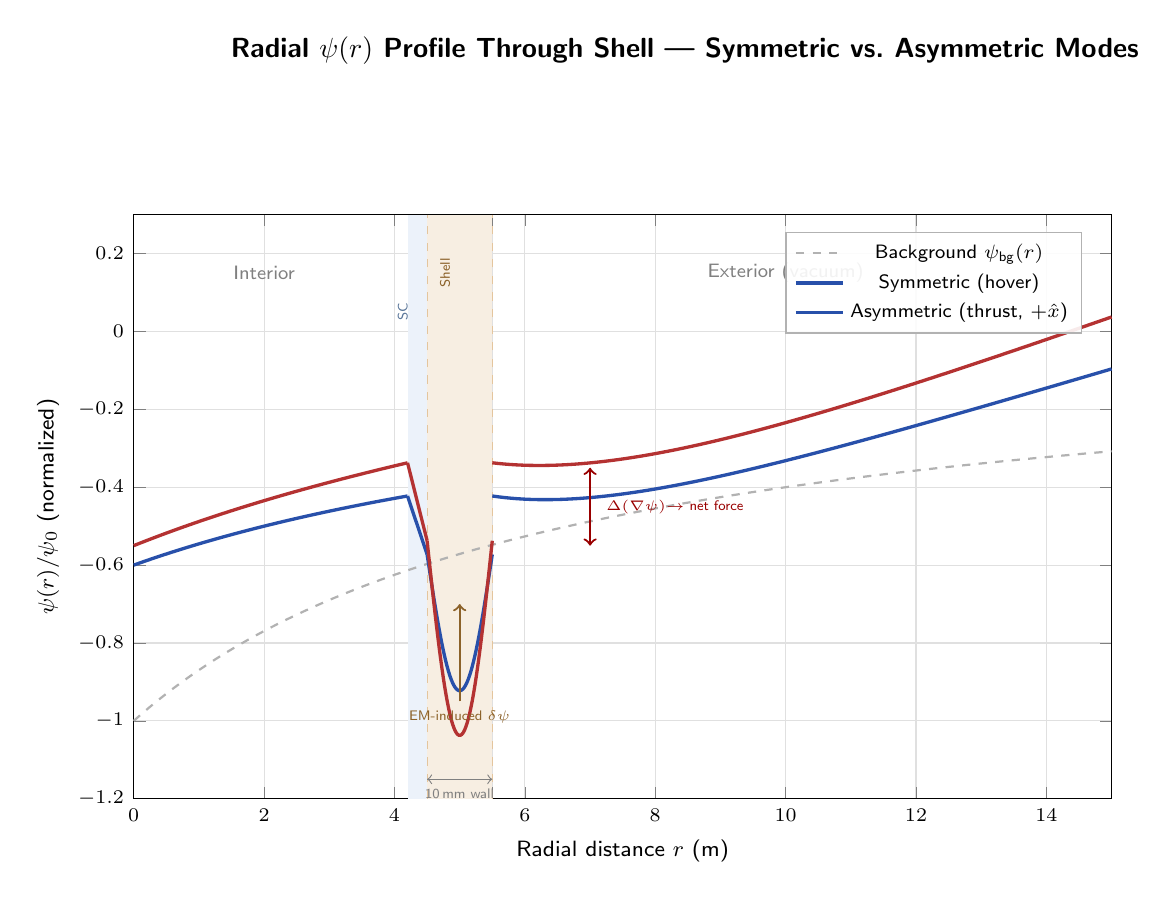
\begin{tikzpicture}

\definecolor{symBlue}{RGB}{40,80,170}
\definecolor{asymRed}{RGB}{180,50,50}
\definecolor{shellRegion}{RGB}{200,140,60}
\definecolor{scRegion}{RGB}{130,170,220}

\begin{axis}[
    width=14cm, height=9cm,
    xmin=0, xmax=15,
    ymin=-1.2, ymax=0.3,
    xlabel={Radial distance $r$ (m)},
    ylabel={$\psi(r) / \psi_0$ (normalized)},
    xlabel style={font=\footnotesize\sffamily},
    ylabel style={font=\footnotesize\sffamily},
    tick label style={font=\scriptsize\sffamily},
    grid=major,
    grid style={black!12},
    legend style={
        font=\scriptsize\sffamily,
        at={(0.97,0.97)},
        anchor=north east,
        draw=black!30,
        fill=white,
        fill opacity=0.9,
        text opacity=1,
    },
    clip=false,
    % Shell region shading
    extra x ticks={4.5,5.5},
    extra x tick labels={},
]

% --- Shell region shading ---
\fill[shellRegion!15] (axis cs:4.5,-1.2) rectangle (axis cs:5.5,0.3);
\draw[shellRegion!50, dashed] (axis cs:4.5,-1.2) -- (axis cs:4.5,0.3);
\draw[shellRegion!50, dashed] (axis cs:5.5,-1.2) -- (axis cs:5.5,0.3);
\node[font=\tiny\sffamily, shellRegion!70!black, rotate=90, anchor=south]
    at (axis cs:5,0.15) {Shell};

% --- Superconductor region ---
\fill[scRegion!15] (axis cs:4.2,-1.2) rectangle (axis cs:4.5,0.3);
\node[font=\tiny\sffamily, scRegion!70!black, rotate=90, anchor=south]
    at (axis cs:4.35,0.05) {SC};

% --- Background potential (no EM, dashed gray) ---
\addplot[black!30, thick, dashed, domain=0:15, samples=200] {
    -1/(1 + x*0.15)
};
\addlegendentry{Background $\psi_\text{bg}(r)$}

% --- Symmetric configuration (hover mode) ---
% Inside shell: deep well from EM energy
% Outside shell: symmetric perturbation decaying as 1/r
\addplot[symBlue, very thick, domain=0:4.2, samples=100] {
    -0.6/(1 + x*0.1)
};
\addplot[symBlue, very thick, domain=4.2:4.5, samples=30] {
    -0.6/(1 + 4.2*0.1) - 0.15*(x-4.2)/0.3
};
\addplot[symBlue, very thick, domain=4.5:5.5, samples=50] {
    -0.6/(1 + 4.2*0.1) - 0.15 - 0.35*sin(deg((x-4.5)*3.14159/1.0))
};
\addplot[symBlue, very thick, domain=5.5:15, samples=100] {
    -0.6/(1 + 4.2*0.1) - 0.15 - 0.0 + 0.15*exp(-(x-5.5)*0.5) + (x-5.5)*0.05
};
\addlegendentry{Symmetric (hover)}

% --- Asymmetric configuration (thrust, +x direction) ---
% Stronger perturbation on thrust side
\addplot[asymRed, very thick, domain=0:4.2, samples=100] {
    -0.55/(1 + x*0.1) + 0.05*x/4.2
};
\addplot[asymRed, very thick, domain=4.2:4.5, samples=30] {
    -0.55/(1 + 4.2*0.1) + 0.05 - 0.2*(x-4.2)/0.3
};
\addplot[asymRed, very thick, domain=4.5:5.5, samples=50] {
    -0.55/(1 + 4.2*0.1) + 0.05 - 0.2 - 0.5*sin(deg((x-4.5)*3.14159/1.0))
};
\addplot[asymRed, very thick, domain=5.5:15, samples=100] {
    -0.55/(1 + 4.2*0.1) + 0.05 - 0.2 - 0.0 + 0.2*exp(-(x-5.5)*0.4)
    + (x-5.5)*0.06
};
\addlegendentry{Asymmetric (thrust, $+\hat{x}$)}

% --- Annotations ---

% EM energy perturbation in shell
\draw[->, shellRegion!70!black, thick]
    (axis cs:5,-0.95) -- (axis cs:5,-0.7);
\node[font=\tiny\sffamily, shellRegion!70!black, below] at (axis cs:5,-0.95)
    {EM-induced $\delta\psi$};

% Gradient difference
\draw[<->, red!60!black, thick]
    (axis cs:7,-0.55) -- (axis cs:7,-0.35);
\node[font=\tiny\sffamily, red!60!black, right] at (axis cs:7.1,-0.45)
    {$\Delta(\nabla\psi)$\\$\to$ net force};

% Interior label
\node[font=\scriptsize\sffamily, black!50] at (axis cs:2,0.15)
    {Interior};
\node[font=\scriptsize\sffamily, black!50] at (axis cs:10,0.15)
    {Exterior (vacuum)};

% Shell wall detail
\draw[<->, black!50, thin] (axis cs:4.5,-1.15) -- (axis cs:5.5,-1.15);
\node[font=\tiny\sffamily, black!50, below] at (axis cs:5,-1.15) {10\,mm wall};

\end{axis}

% ============================================================
% TITLE
% ============================================================
\node[font=\normalsize\sffamily\bfseries, anchor=south] at (7,9.2)
    {Radial $\psi(r)$ Profile Through Shell --- Symmetric vs.\ Asymmetric Modes};

\end{tikzpicture}
\end{document}
